\documentclass[a4paper,11pt]{article}

\usepackage{latexsym}
\usepackage{graphicx}
\usepackage{float}
\usepackage[margin=2cm]{geometry}
\usepackage{lscape}
\usepackage{underscore}
\usepackage{amsmath}
\usepackage{blindtext}
\usepackage{listings}
\usepackage{xcolor}
\usepackage{mathtools}

\usepackage[all]{nowidow}

\usepackage[LY1]{fontenc}
\usepackage[utf8x]{inputenc}
\usepackage{polski}
\usepackage[lf,enc=t1]{berenis}

\DeclareTextCompositeCommand{\k}{LY1}{a}
  {\oalign{a\crcr\noalign{\kern-.27ex}\hidewidth\char7}}

\usepackage{color}
\definecolor{lightgray}{rgb}{.9,.9,.9}
\definecolor{darkgray}{rgb}{.4,.4,.4}
\definecolor{purple}{rgb}{0.65, 0.12, 0.82}

\lstdefinelanguage{JavaScript}{
  keywords={typeof, new, true, false, catch, function, return, null, catch, switch, var, if, in, while, do, else, case, break},
  keywordstyle=\color{blue}\bfseries,
  ndkeywords={class, export, boolean, throw, implements, import, this},
  ndkeywordstyle=\color{darkgray}\bfseries,
  identifierstyle=\color{black},
  sensitive=false,
  comment=[l]{//},
  morecomment=[s]{/*}{*/},
  commentstyle=\color{purple}\ttfamily,
  stringstyle=\color{red}\ttfamily,
  morestring=[b]',
  morestring=[b]"
}


\lstset{
    language=JavaScript,
    frame=tb, % draw a frame at the top and bottom of the code block
    tabsize=4, % tab space width
    showstringspaces=false, % don't mark spaces in strings
    numbers=left, % display line numbers on the left
    backgroundcolor=\color{black!5}, 
   % commentstyle=\color{green}, % comment color
    keywordstyle=\color{blue}, % keyword color
    stringstyle=\color{red}, % string color  
    inputencoding=utf8x,
    extendedchars=\true,
    literate={ą}{{\k{a}}}1
             {Ą}{{\k{A}}}1
             {ę}{{\k{e}}}1
             {Ę}{{\k{E}}}1
             {ó}{{\'o}}1
             {Ó}{{\'O}}1
             {ś}{{\'s}}1
             {Ś}{{\'S}}1
             {ł}{{\l{}}}1
             {Ł}{{\L{}}}1
             {ż}{{\.z}}1
             {Ż}{{\.Z}}1
             {ź}{{\'z}}1
             {Ź}{{\'Z}}1
             {ć}{{\'c}}1
             {Ć}{{\'C}}1
             {ń}{{\'n}}1
             {Ń}{{\'N}}1
	     {*}{\normalfont{*}}1,
}


\begin{document}
\begin{titlepage}


\newcommand{\HRule}{\rule{\linewidth}{0.5mm}}
\center

\textsc{\LARGE Politechnika Wrocławska}\\[1.5cm]
\textsc{\LARGE Grafika komputerowa}\\[0.5cm]

\HRule \\[0.5cm]
{ \huge \bfseries Projekt zaliczeniowy: \\[0.3cm]WebGL -podstawy oraz fraktal 2D}\\[0.5cm] 
\HRule \\[1.5cm]

\begin{flushleft} \large
 
\emph{Autor:}\\
 
Bartosz  \textsc{Pogoda} 225988 \\
 
\end{flushleft}
%\end{minipage}
 
%\begin{minipage}{0.4\textwidth}
\begin{flushright} \large
 
\emph{Prowadzący:} \\
mgr inż. Szymon \textsc{Datko} 
 
\end{flushright}
%\end{minipage}\\[4cm]
 
\vfill
{\large 15 stycznia 2018}\\[3cm] 
 
 
\end{titlepage}

\tableofcontents
\newpage

\section{Wstęp teoretyczny}

WebGL jest biblioteką pozwalającą na renderowanie grafiki 2D oraz 3D przy użyciu języka JavaScript. Wyrenderowane sceny są prezentowane w przeglądarce przy pomocu elementu <canvas> wprowadzonego wraz ze standardem HTML5. Implementacja WebGL zapewnia wszystkie możliwośći biblioteki OpenGL poznanej na zajęciach, tj.  renderowanie 2D, renderowanie 3D, oświetlanie, teksturowanie.


\section{Założenia projektowe}

W ramach projektu zostały zrealizowane następujące zadania:
\begin{itemize}
\item zapoznanie się z instrukcją dostępną na stronie kursu,
\item wyrysowanie czworościanu,
\item warunek blokujący funkcję uruchom,
\item wyrenderowanie fraktala 2D,
\item umożliwienie regulacji parametrów renderowania przy pomocy UI.
\end{itemize}

\section{Realizacja projektu}

\subsection{Zapoznanie się z instrukcją}

Przeczytanie instrukcji zamieszczonej na stronie kursu oraz przetestowanie załączonych przykładów pozwoliło na poznanie technik realizacji różnych możliwości biblioteki OpenGL, poznanych na wcześniejszych zajęciach, w obrębie technologii WebGL. 

\subsubsection {Kontekst graficzny}

Biblioteka WebGL oferuje interfejs WebGLRenderingContext, który zawiera wszelkie operacje potrzebne do rysowania scen 2D oraz 3D w ramach elementu <canvas>. Przed rozpoczęciem renderowania scen należy pobrać kontekst graficzny.

\begin{lstlisting}[caption= Pobranie kontekstu graficznego]
var canvas = document.getElementById('myCanvas');
var gl_ctx = canvas.getContext('webgl');
\end{lstlisting}

Tak pobrany kontekst udostępnia wszystkie możliwości biblioteki WebGL, a więc między innymi:
\begin{itemize}
\item pozyskiwanie informacji o stanie,
\item zarządzanie buforami,
\item zarządzanie teksturami,
\item zarządzanie programami oraz shaderami,
\item zarządzanie atrybutami,
\item renderowanie.
\end{itemize}


\subsubsection{Bufory wierzchołków oraz indeksów}

Bardzo ważne z punktu widzenia dalszej realizacji projektu było opanowanie renderowania obiektów 3D (oraz analogicznie 2D) podając ich wierzchołki. W WebGL tworzy się dwa bufory. Jeden z buforów zawiera współrzędne kolejnych wierzchołków w przestrzeni, wraz z informacją o kolorach przypisanych tym wierzchołkom. Drugi bufor określa kolejność występowania wierzchołków zdefiniowanych w pierwszym buforze (podawane jako indeksy 0, 1, ...) w rysowanych figurach. Poniżej zostały zamieszczone dwie przykładowe tablice, które mogą zostać użyte jako bufory w celu wyrysowania na scenie 3D czworościanu.

\begin{lstlisting}[caption=Definicja tablicy opisującej bufor wierzchołków dla czworościanu]
var tetahedronVerticles = [
      1, 1, 1,
      1, 0, 0,

      -1, -1, 1,
      0, 1, 0,

      -1, 1, -1,
      0, 0, 1,

      1, -1, -1,
      1, 1, 0
];
\end{lstlisting}

\begin{lstlisting}[caption=Definicja tablicy opisującej bufor indeksów dla czworościanu]
  var tetahedronFaces = [
      0, 1, 2,
      0, 2, 3,
      0, 1, 3,
      1, 2, 3,
];
\end{lstlisting}

\subsubsection{Rejestracja buforów}

Wyżej zdefiniowane struktury nie są jednak widziane jako bufory w bibliotece WebGL. Tak zdefiniowane tablice zawierają wszelkie potrzebne dane, jednak bufory muszą zostać utworzone oraz zarejestrowane przy użyciu kontesktu graficznego (typu \textit{WebGLRenderingContext}).

\begin{lstlisting}[caption=Utworzenie oraz przypięcie bufora wierzchołków]
_tetahedronVertexBuffer = gl_ctx.createBuffer();

gl_ctx.bindBuffer(gl_ctx.ARRAY_BUFFER, _tetahedronVertexBuffer);

gl_ctx.bufferData(gl_ctx.ARRAY_BUFFER, 
                         new Float32Array(tetahedronVerticles),
                         gl_ctx.STATIC_DRAW);
\end{lstlisting}

Bufor dla kontekstu \textit{gl_ctx} został utworzony za pomocą metody \textit{createBuffer}. Następnie bufor ten został przypisany do kontekstu wraz z informacją o typie. Ostatecznie bufor został wypełniony danymi zawartymi we wcześniej zdefiniowanej tablicy \textit{tetahedronVerticles}.

\newpage
\begin{lstlisting}[caption=Utworzenie oraz przypięcie bufora indeksów]
_tetahedronFacesBuffer = gl_ctx.createBuffer();

gl_ctx.bindBuffer(gl_ctx.ELEMENT_ARRAY_BUFFER, 
				   		_tetahedronFacesBuffer);

gl_ctx.bufferData(gl_ctx.ELEMENT_ARRAY_BUFFER,
				   		new Uint16Array(tetahedronFaces),
				   		gl_ctx.STATIC_DRAW);
\end{lstlisting}

W sposób analogiczny został utworzony oraz przypisany bufor indeksów. Warto zwrócić uwagę na typ \textit{WebGLRenderingContext.ELEMENT_ARRAY_BUFFER}, który przekazuje informację, że dany bufor zawiera informację o kolejności wierzchołków, a nie tak jak w przypadku \textit{WebGLRenderingContext.ARRAY_BUFFER} - o położeniu wierzchołków oraz ich kolorach.

\subsection{Wyrysowanie czworościanu}

Skrypt zamieszczony na stronie kursu został zmodyfikowany tak, aby na ekranie został wyrysowany czworościan. W tym celu współrzedne przykładowego czworościanu (1,1,1), (-1,-1,1), (-1,1,-1), (1,-1,-1) zostały zapisane w buforach, tak jak zdefiniowano na wyżej zamieszczonych listingach.

\begin{lstlisting}[caption=Wyrysowanie elemetów zawartych w buforach]
gl_ctx.drawElements(gl_ctx.TRIANGLES, 4*3, 
					gl_ctx.UNSIGNED_SHORT, 0);
gl_ctx.flush();
\end{lstlisting}

Czworościan został uzyskany poprzez narysowanie \textbf{czterech} \textbf{trójkątów} (każdy zdefiniowany przez \textbf{trzy} wierzchołki). Pogrubione parametry są istotne i można je odnaleźć przy wywołaniu funkcji \textit{drawElements}. Warto zaznaczyć, że funkcja rysuje obiekty na podstawie aktualnie przypisanych buforów.

\begin{figure}[H]
\centering
 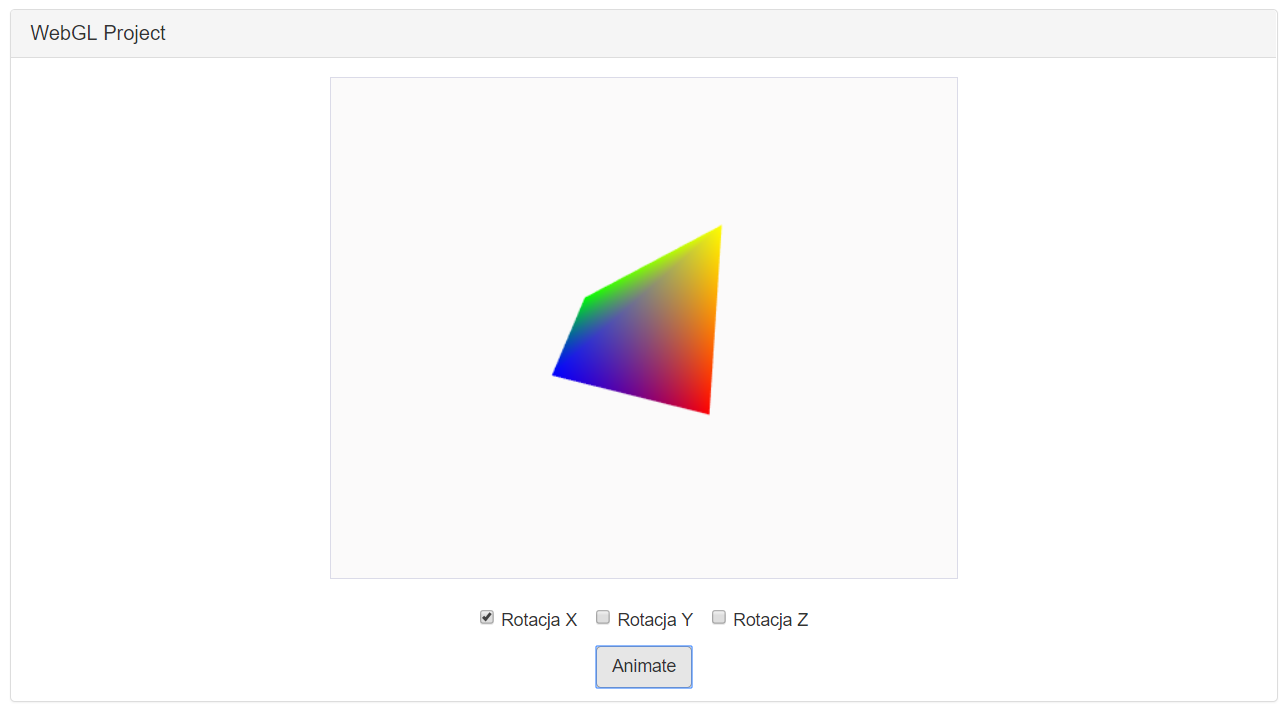
\includegraphics[height=9cm]{czworoscian.PNG}
\caption{Czworościan wyrenderowany w oknie przeglądarki}
\end{figure}


\begin{figure}[H]
\centering
 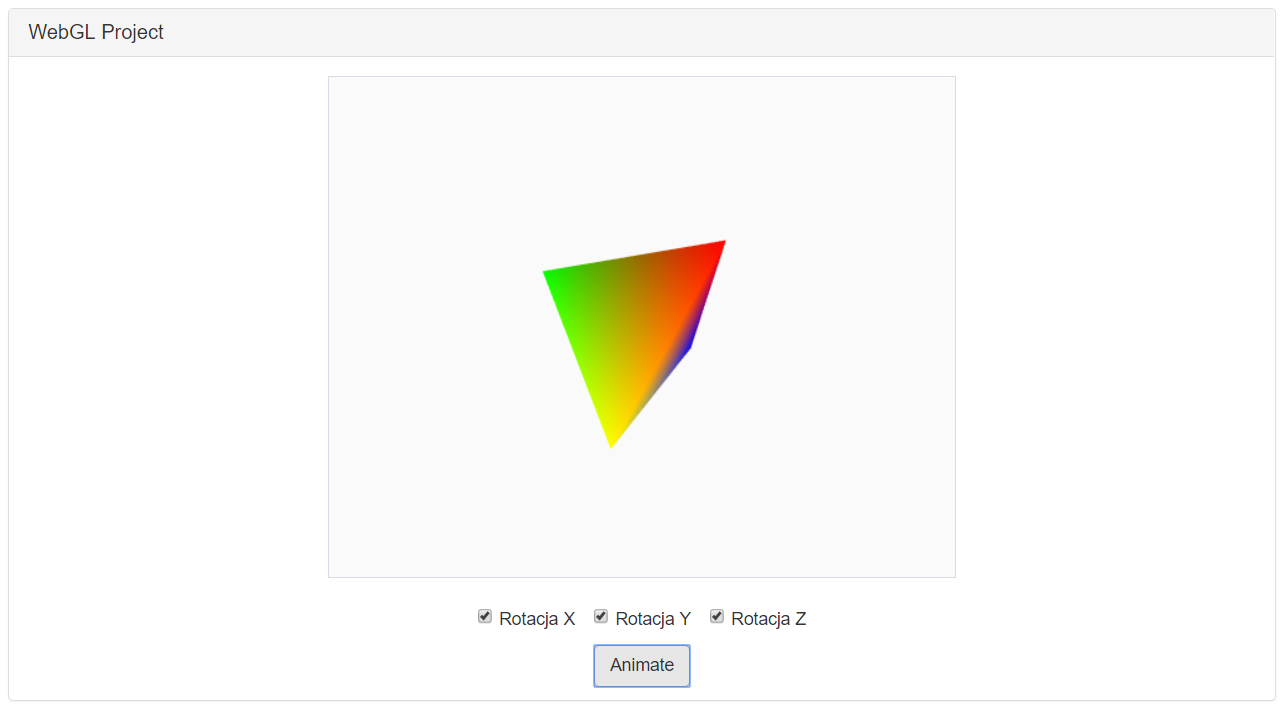
\includegraphics[height=9cm]{czworoscian2.PNG}
\caption{Czworościan w innej fazie rotacji}
\end{figure}

\subsection{Warunek blokujący funkcję uruchom}

Przykład, na podstawie którego została stworzona wyżej opisana funkcjonalność, zawierał pewną niedoskonałość (chociaż można by równie dobrze nazwać ją "dodatkową funkcjonalnością") związaną z przyśpieszaniem animacji każdorazowo po wciśnięciu przycisku "Animate".

Niedoskonałość wynikała z każdorazowego dodawania funkcji zwrotnej przy wciśnięciu "Animate" za pomocą funkcji \textit{requestAnimationFrame} obiektu typu \textit{Window}. Funkcja ta przy wywołaniu rejestruje kolejną funkcję (zadaną argumentem), która zostanie uruchomiona przed przerysowaniem zawartości ekranu przez przeglądarkę, czyli zazwyczaj około 60 razy na sekundę.  Rejestrowanie kolejnych callback'ów za każdym razem powodowało wywołanie tej samej funkcji wiele razy, co skutkowało widocznym zwielokrotnieniem szybkości animacji.

Przykładowym obejściem problemu, które zostało zrealizowane w ramach projektu, było utworzenie flagi, która zostaje ustawiona przy pierwszym uruchomieniu animacji. Przy następnych wciśnięciach przycisku "Animate" funkcje zwrotne nie są rejestrowane na nowo, ze względu na wykrycie ustawionej flagi.


\begin{lstlisting}[caption=Realizacja obejścia problemu przyśpieszania animacji]
var alreadyAnimating = false;

function gl_draw() {
    // logika rysowania sceny 

    var animate = function (time) {
      // logika animacji

      window.requestAnimationFrame(animate);
   };

  if(!alreadyAnimating) {
    animate(0);
    alreadyAnimating = true;
  }
}
\end{lstlisting}


\subsection{Wyrenderowanie fraktala 2D}

Projekt został rozbudowany o wyrenderowanie dywanu Sierpińskiego. Cała logika renderowania została umieszczona w klasie \textit{CarpetDrawer}, której deklaracje metod zostały przedstawione na poniższym diagramie.

\begin{figure}[H]
\centering
 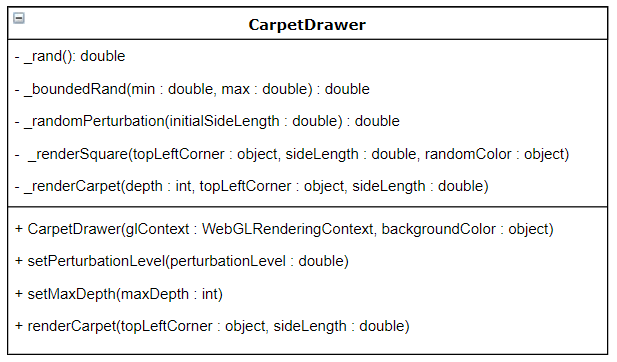
\includegraphics[height=7cm]{uml.PNG}
\caption{Deklaracja metod klasy CarpetDrawer}
\end{figure}

\subsubsection{Losowość}

W pierwszej kolejności zostały zdefiniowane metody służace do generowania liczb pseudolosowych, które następnie zostały użyte do losowania kolorów wierzchołków oraz zaburzeń we współrzędnych wierzchołków - czyli perturbacji.

\subsubsection{Renderowanie kwadratu}

Kluczowym etapem implementacji było utworzenie metody odpowiedzialnej za wyrysowanie na ekranie kwadratu w zadanym miejscu, o zadanej długości boku oraz trybie kolorowania. 



\begin{lstlisting}[caption=Realizacja funkcji renderującej pojedyńczy kwadrat]
// Renders square for given topLeftCorner, sideLength. 
// It has random color if randomColor is set true, 
// backgoundColor otherwise 
_renderSquare(topLeftCorner, sideLength, randomColor) {
  var _rand = this._rand;
  var glContext = this.glContext;
  var backgroundColor = this.backgroundColor;

  if (randomColor) {

    var squareVerticles = [
      topLeftCorner.x, topLeftCorner.y,
      _rand(), _rand(), _rand(),
      topLeftCorner.x + sideLength, topLeftCorner.y,
      _rand(), _rand(), _rand(),
      topLeftCorner.x + sideLength, topLeftCorner.y - sideLength,
      _rand(), _rand(), _rand(),
      topLeftCorner.x, topLeftCorner.y - sideLength,
      _rand(), _rand(), _rand()
    ];

  } else {
    var squareVerticles = [
      topLeftCorner.x, topLeftCorner.y,
      backgroundColor.r, backgroundColor.g, backgroundColor.b,
      topLeftCorner.x + sideLength, topLeftCorner.y,
      backgroundColor.r, backgroundColor.g, backgroundColor.b,
      topLeftCorner.x + sideLength, topLeftCorner.y - sideLength,
      backgroundColor.r, backgroundColor.g, backgroundColor.b,
      topLeftCorner.x, topLeftCorner.y - sideLength,
      backgroundColor.r, backgroundColor.g, backgroundColor.b,
    ];
  }

  var squareVertexBuffer = glContext.createBuffer();
  glContext.bindBuffer(glContext.ARRAY_BUFFER,
					   squareVertexBuffer);
  glContext.bufferData(glContext.ARRAY_BUFFER, 
					   new Float32Array(squareVerticles), 
				   	   glContext.STATIC_DRAW);

  var squareFaces = [
    0, 1, 2,
    0, 2, 3
  ];

  var squareFacesBuffer = glContext.createBuffer();
  glContext.bindBuffer(glContext.ELEMENT_ARRAY_BUFFER,
					    squareFacesBuffer);
  glContext.bufferData(glContext.ELEMENT_ARRAY_BUFFER, 
					    new Uint16Array(squareFaces), 
					    glContext.STATIC_DRAW);

  gl_ctx.vertexAttribPointer(_position, 2, gl_ctx.FLOAT, false, 
					   	 4 * (2 + 3), 0);
  gl_ctx.vertexAttribPointer(_color, 3, gl_ctx.FLOAT, false, 
					         4 * (2 + 3), 2 * 4);

  glContext.drawElements(glContext.TRIANGLES, 2 * 3, 
					     glContext.UNSIGNED_SHORT, 0);
}
\end{lstlisting}
\newpage
\subsubsection{Renderowanie dywanu Sierpińskiego}

Po zaimplementowaniu oraz przetestowaniu poprawności działania powyższych funkcji pomocniczych, zostały utworzone funkcje \textit{renderCarpet} oraz \textit{_renderCarpet}. Funkcja \textit{renderCarpet} startuje rekurencyjną procedurę renderowania kolejnych poziomów głębokości dywanu Sierpińskiego. W każdym etapie rekurencji wyrenderowanych zostało osiem kwadratów dookoła wypełnionych losowymi kolorami oraz jeden kwadrat wewnątrz wypełniony kolorem tła. Do wyliczonych pozycji kwadratów zostały zaaplikowane losowe perturbacje.

\begin{lstlisting}[caption=Definicja funkcji renderCarpet]
renderCarpet(topLeftCorner, sideLength) {
  this._renderCarpet(0, topLeftCorner, sideLength)
  this.glContext.flush();
}
\end{lstlisting}

\begin{lstlisting}[caption=Definicja funkcji rekurencyjnej _renderCarpet]
_renderCarpet(depth, topLeftCorner, sideLength) {
  if (depth >= this.maxDepth) return;

  var subSquareSideLength = sideLength / 3;

  // Draw empty square
  var emptySquareTopLeftCorner = {
    x: topLeftCorner.x + subSquareSideLength,
    y: topLeftCorner.y - subSquareSideLength
  };
  this._renderSquare({
    x: topLeftCorner.x + subSquareSideLength,
    y: topLeftCorner.y - subSquareSideLength
  }, subSquareSideLength, false);

  // Draw remaining (randomly filled) squares
  for (var i = 0; i < 3; i++) {
    for (var j = 0; j < 3; j++) {
      if (!(i == 1 && i == j)) { // skip one which should be empty
        var deformation = this._randomPerturbation
										(subSquareSideLength);
        var subSquareTopLeftCorner = {
          	x: topLeftCorner.x +
		 (i * subSquareSideLength) + deformation,
			y: topLeftCorner.y - 
		(j * subSquareSideLength) + deformation
        };

        this._renderSquare(subSquareTopLeftCorner, 
						subSquareSideLength, true);
        // render carpet recursive call
        this._renderCarpet(depth + 1, subSquareTopLeftCorner, 
						subSquareSideLength);
      }
    }
  }
}
\end{lstlisting}

\subsection{Umożliwienie regulacji parametrów renderowania przy pomocy UI}

W ramach interfejsu użytkownika utworzono dwa suwaki - do sterowania poziom perturbacji oraz głębokością wywołań rekurencyjnych. Suwaki zostały utworzone przy pomocy biblioteki jQueryUI. 

\begin{lstlisting}[caption=Utworzenie suwaka dla zmian poziomu perturbacji]
var perturbationPreview = $("#perturbationPreview");
$("#perturbationSlider").slider({
  range: "min",
  min: 0,
  max: 150,
  value: 1,
  create: function() {
    perturbationPreview.text($(this).slider("value") / 100);
  },
  slide: function(event, ui) {
    perturbationPreview.text(ui.value / 100);
  }
});
\end{lstlisting}

Parametry ustawione za pomocą suwaków są przekazywane do modelu (obiektu klasy \textit{CarpetDrawer}) po wciśnięciu przycisku "Render". Następnie wywoływana jest funkcja \textit{renderCarpet}, która renderuje dywan o lewym górnym wierzchołku (-1, 1) i długości boku 2, co przy domyślnym ustawieniu pozycji "kamery" skutkuje pokryciem całego obszaru rysowania.

\begin{lstlisting}[caption=Metoda wywołująca się przy nacisnięciu przycisku "Render"]
function gl_draw() {
  var backgroundColor = {
    r: 0.984,
    g: 0.980,
    b: 0.980
  };

  gl_ctx.clearColor(backgroundColor.r, backgroundColor.g, 
					backgroundColor.b, 1.0);

  let carpetDrawer = new CarpetDrawer(gl_ctx, backgroundColor);
  carpetDrawer.setPeturbationLevel($("#perturbationPreview")
										.text());
  carpetDrawer.setMaxDepth($("#depthPreview").text());

  carpetDrawer.renderCarpet({ x: -1, y: 1 }, 2);
}
\end{lstlisting}


\section{Zrzuty ekranu}

\begin{figure}[H]
\centering
 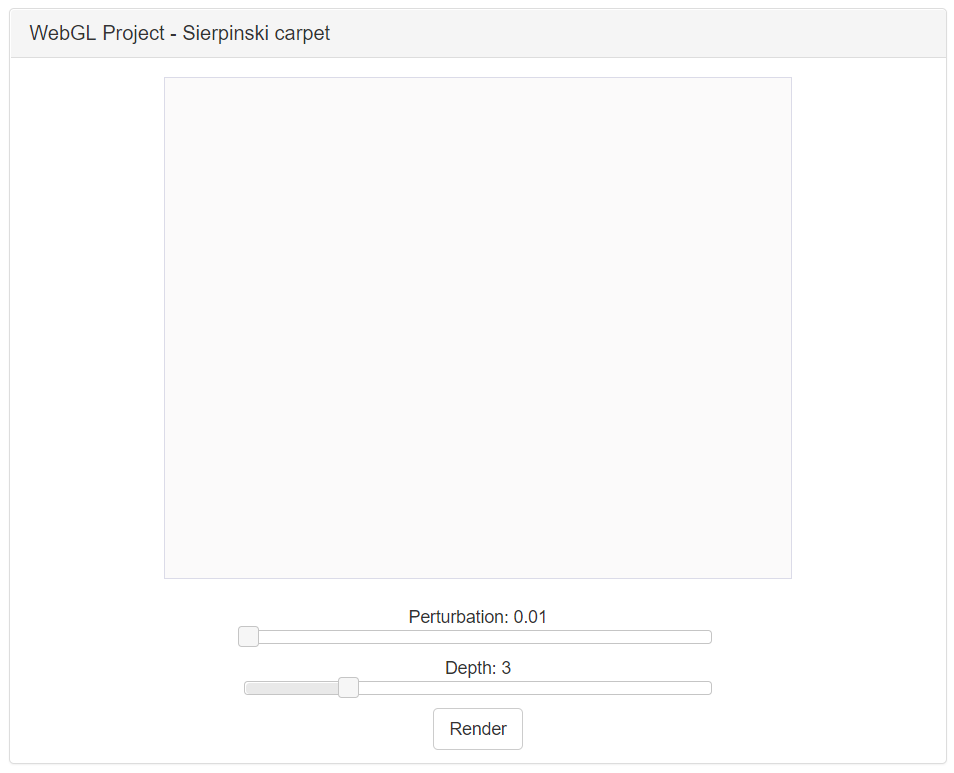
\includegraphics[height=10cm]{sierp.PNG}
\caption{Interfejs użytkownika}
\end{figure}



\begin{figure}[H]
\centering
 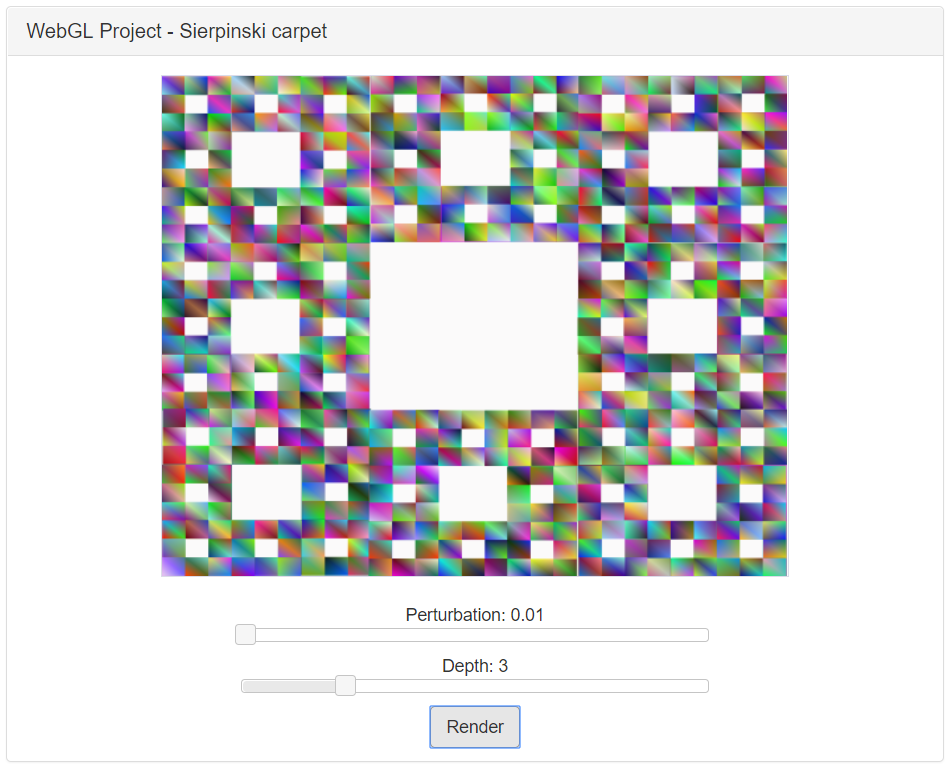
\includegraphics[height=10cm]{pert1.PNG}
\caption{Wyrenderowany podstawowy dywan Sierpińskiego, o bardzo niskim poziomie perturbacji}
\end{figure}



\begin{figure}[H]
\centering
 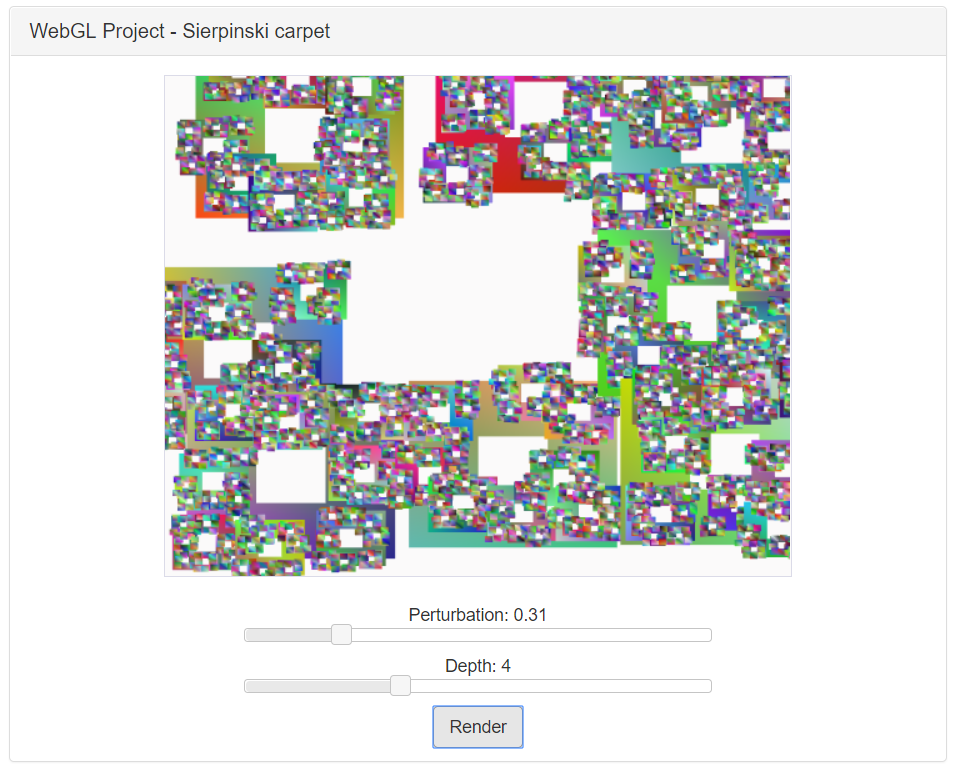
\includegraphics[height=10cm]{pert2.PNG}
\caption{Wyrenderowany dywan Sierpińskiego, o średnim poziomie perturbacji oraz głębokości 4}
\end{figure}

\begin{figure}[H]
\centering
 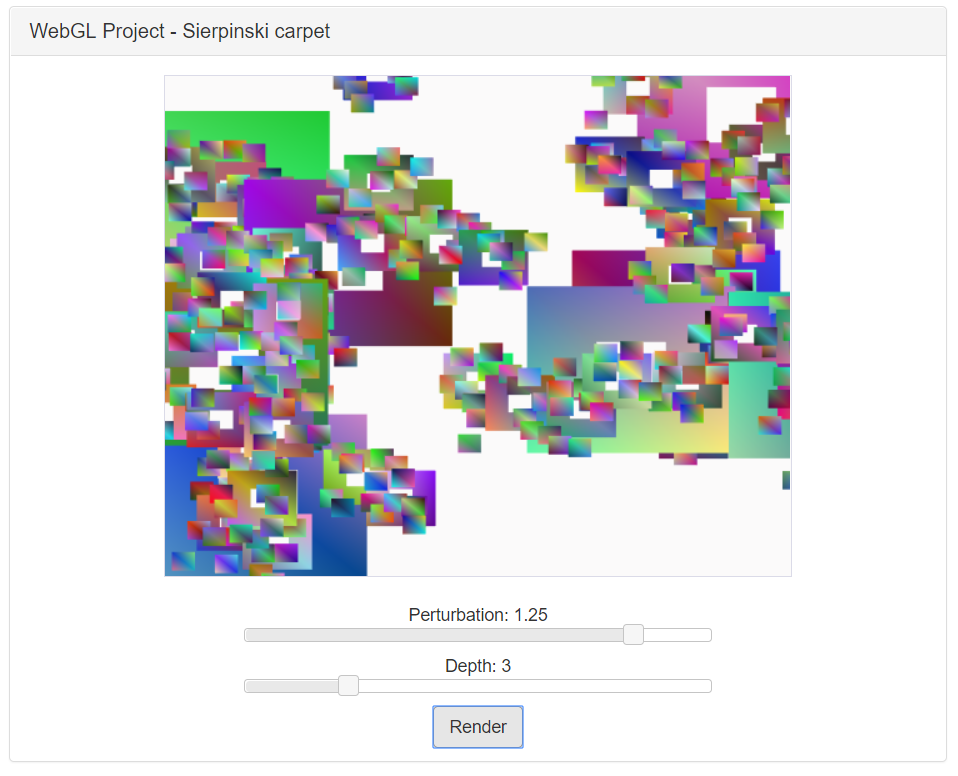
\includegraphics[height=10cm]{pert3.PNG}
\caption{Wyrenderowany dywan Sierpińskiego, o wysokim poziomie perturbacji oraz głębokości 3}
\end{figure}

\begin{figure}[H]
\centering
 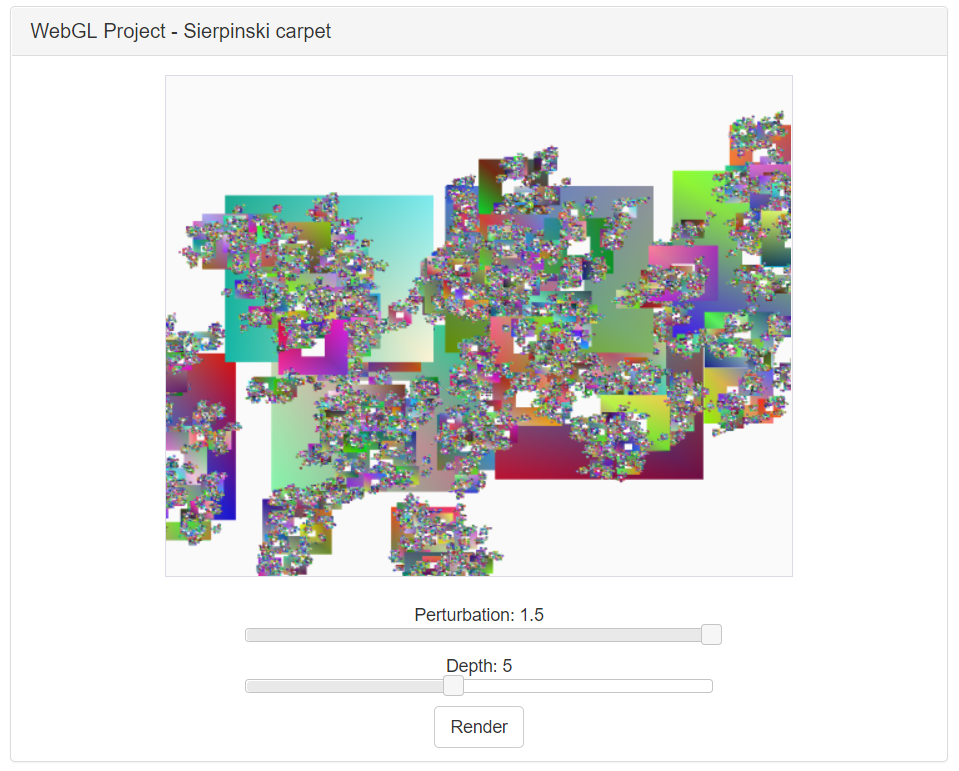
\includegraphics[height=10cm]{pert4.PNG}
\caption{Wyrenderowany dywan Sierpińskiego, o bardzo wysokim poziomie perturbacji oraz głębokości 5}
\end{figure}

\section{Podsumowanie}

Realizacja projektu pozwoliła mi nabyć wiedzę teoretyczną oraz praktyczną na temat technologii WebGL.


\begin{thebibliography}{99}
\bibitem{pa} Instrukcja laboratoryjna. http://www.zsk.ict.pwr.wroc.pl/zsk/dyd/intinz/gk/lab/cw_8_dz/
\bibitem{pa} WebGL API. https://developer.mozilla.org/en-US/docs/Web/API/WebGL_API
\bibitem{pa} Różnice WebGL i OpenGL. https://www.khronos.org/webgl/wiki/WebGL_and_OpenGL_Differences
\bibitem{pa} Kontekst graficzny. https://developer.mozilla.org/en-US/docs/Web/API/WebGLRenderingContext
\end{thebibliography}


\end{document}